%%%%%%%%%%%%%%%%%%%%%%%%%%%%%%%%%%%%%%%%%
% University/School Laboratory Report
% LaTeX Template
% Version 3.1 (25/3/14)
%
% This template has been downloaded from:
% http://www.LaTeXTemplates.com
%
% Original author:
% Linux and Unix Users Group at Virginia Tech Wiki 
% (https://vtluug.org/wiki/Example_LaTeX_chem_lab_report)
%
% License:
% CC BY-NC-SA 3.0 (http://creativecommons.org/licenses/by-nc-sa/3.0/)
%
%%%%%%%%%%%%%%%%%%%%%%%%%%%%%%%%%%%%%%%%%

%----------------------------------------------------------------------------------------
%	PACKAGES AND DOCUMENT CONFIGURATIONS
%----------------------------------------------------------------------------------------

\documentclass[UTF8]{article}

\usepackage[version=3]{mhchem} % Package for chemical equation typesetting
\usepackage{siunitx} % Provides the \SI{}{} and \si{} command for typesetting SI units
\usepackage{graphicx} % Required for the inclusion of images
\usepackage{natbib} % Required to change bibliography style to APA
\usepackage{amsmath} % Required for some math elements 
\usepackage{ctex}
\usepackage{listings}
\usepackage{xcolor}
\usepackage{url}
\setlength\parindent{0pt} % Removes all indentation from paragraphs

\renewcommand{\labelenumi}{\alph{enumi}.} % Make numbering in the enumerate environment by letter rather than number (e.g. section 6)

%\usepackage{times} % Uncomment to use the Times New Roman font

%----------------------------------------------------------------------------------------
%	DOCUMENT INFORMATION
%----------------------------------------------------------------------------------------

\title{\textbf{数字逻辑实验} \\ \textbf{点亮数字人生} \\ \textbf{实验报告}} % Title

\author{数字逻辑实验A班  \quad 计86 \\ 任一 2018011423} % Author name

\date{\today} % Date for the report


\lstset{
    % backgroundcolor=\color{red!50!green!50!blue!50},%代码块背景色为浅灰色
    rulesepcolor= \color{gray}, %代码块边框颜色
    % breaklines=true,  %代码过长则换行
    numbers=left, %行号在左侧显示
    numberstyle= \small,%行号字体
    keywordstyle= \color{blue},%关键字颜色
    commentstyle=\color{gray}, %注释颜色
    frame=shadowbox%用方框框住代码块
}
\begin{document}

\maketitle % Insert the title, author and date

% \begin{center}
% \begin{tabular}{l r}
% Date Performed: & January 1, 2012 \\ % Date the experiment was performed
% Partners: & James Smith \\ % Partner names
% & Mary Smith \\
% Instructor: & Professor Smith % Instructor/supervisor
% \end{tabular}
% \end{center}

% \begin{center}
%     \begin{tabular}{|l | r|}
%     \hline

%         \multicolumn{2}{|c|}{实验环境} \\ \hline
%         操作系统: & Windows10家庭版 18362.72 \\ \hline% Date the experiment was performed
%         QuartusII版本: & Quartus II 13.0 sp1 \\ \hline% Partner names

%         ModelSim版本: & Modelsim SE-64 10.7 \\ \hline% Instructor/supervisor

%     \end{tabular}
% \end{center}
\begin{center}
    \begin{tabular}{l  r}
    \hline

        \multicolumn{2}{c}{实验环境} \\ \hline
        操作系统: & Windows10家庭版 18362.72 \\ \hline% Date the experiment was performed
        QuartusII版本: & Quartus II 13.0 sp1 \\ \hline% Partner names

        ModelSim版本: & Modelsim SE-64 10.7 \\ \hline% Instructor/supervisor

    \end{tabular}
\end{center}
% % If you wish to include an abstract, uncomment the lines below
% \begin{abstract}
% Abstract text
% \end{abstract}

% \section*{实验环境}
% 操作系统: Windows10家庭版 18362.720 \\
% QuartusII版本: Quartus II 13.0 sp1 \\
% ModelSim版本: Modelsim SE-64 10.7\\

% 基本要求:P100 5.1.6,代码在 P129 附录C   点亮数字人生例程

% 提高要求:P101 5.1.7,要求点亮三个数码管(至少要使用一个不带译码的数码管),这三个数码管

%                  分别显示奇数列、偶数列和自然数列,通过CLK控制数列变化并且有RST复位功能

% CPLD引脚:P126 附录B

% 本次实验只做提高要求

% 提交实验报告时间: 网络学堂中指定的时间窗口,过期酌情减分
% 请同学们在第五周的周五前完成第一个实验,在网络学堂作业处,提交一个压缩文件,其中包括实验代码和仿真 testbench,和以仿真结果截图加上实验说明(具体内容可以参考实验指导书上“实验报告内容”)为主构成的实验报告,每位同学一个压缩文件提交网络学堂。

\newpage

%----------------------------------------------------------------------------------------
%	SECTION 1
%----------------------------------------------------------------------------------------

\section{实验概述}
\qquad 本实验实现了使用VHDL语言,控制FPGA以显示数字数列,分别能够显示自然数列(16进制与10进制)、偶数列和奇数列。
在本地仿真后,本实验在JieLabs 在线实验平台上进行了进一步的仿真和测试,达到了预期结果。


\qquad 其中,DigitalLife文件夹下为本地测试的实验文件。
在本文件夹的DigitalLife.vhd文件中,我实现了自然数数列、偶数列、奇数列对应的带译码的的数码管和不带译码的数码管共6种输出。DigitalLife\_tb.vhd则是用来测试的testbench文件。


\qquad 此外,DigitalLife\_Online文件夹下,有JieLabs在线实验平台上,本实验使用的仿真代码。考虑到在线实验平台的FPGA只有16个可用的管脚,在本文件夹下的VHDL文件中,本实验选择实现了不带译码的
自然数数列、带译码的偶数列和奇数列。






% % If you have more than one objective, uncomment the below:
% \begin{description}
% \item[First Objective] \hfill \\
% Objective 1 text
% \item[Second Objective] \hfill \\
% Objective 2 text
% \end{description}

% \subsection{Definitions}
% \label{definitions}
% \begin{description}
% \item[Stoichiometry]
% The relationship between the relative quantities of substances taking part in a reaction or forming a compound, typically a ratio of whole integers.
% \item[Atomic mass]
% The mass of an atom of a chemical element expressed in atomic mass units. It is approximately equivalent to the number of protons and neutrons in the atom (the mass number) or to the average number allowing for the relative abundances of different isotopes. 
% \end{description} 
 
%----------------------------------------------------------------------------------------
%	SECTION 2
%----------------------------------------------------------------------------------------

\section{实验结果}
\subsection{仿真截图}



\subsubsection{DigitalLife(本地版本)仿真结果}
\begin{figure}[h]
    \centering
    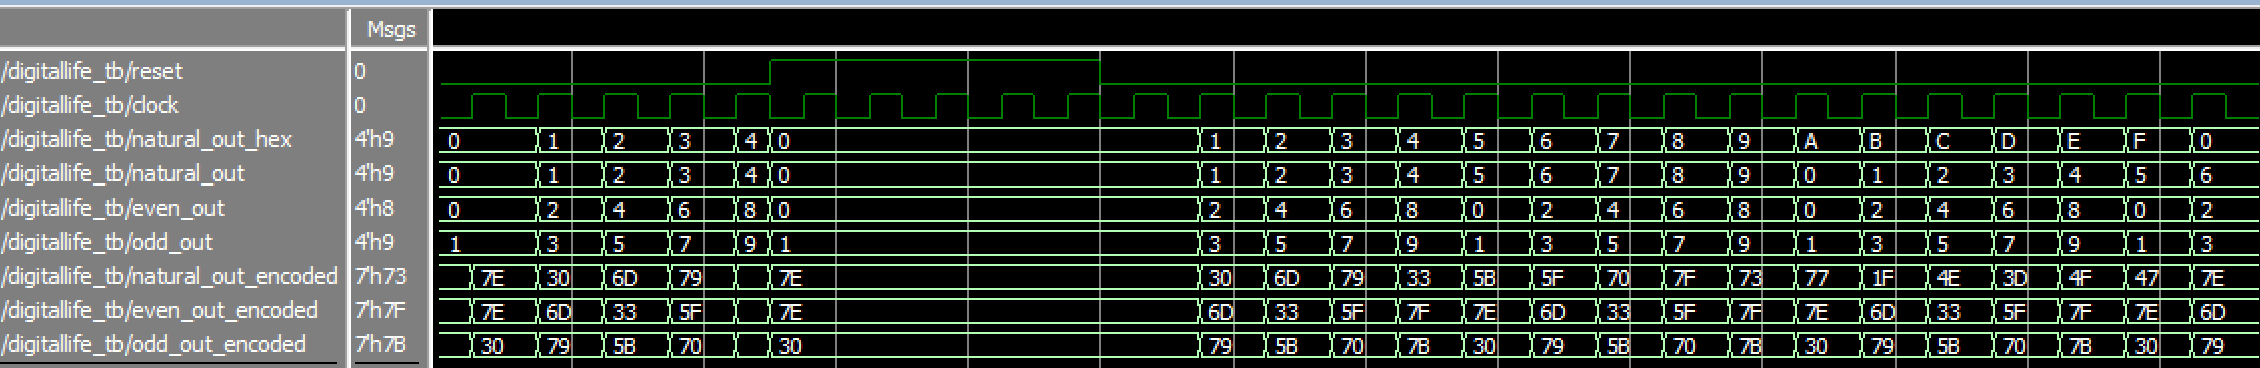
\includegraphics[width=\textwidth]{DL_testbench.png}
    \caption{testbench对DigitalLife文件夹下的文件进行的仿真结果波形图 (放大后清晰可见)}
\end{figure}

\qquad 在上图中,可以看到随着clock信号每次上升沿的出现,各个数列(十六进制自然数列,十进制自然数列、奇数列、偶数列)都发生一次变化。在reset信号从0变为1时,
各信号回到了初始状态,reset信号从1变为0时,各信号继续随时钟变化而变化。其中后三个信号为编码后的数列,对应
没有译码的数码管使用,在本次仿真中其数值没有具体含义。\footnote{为什么图中第一次遇到上升沿时,波形没有变化?详见3.1中的说明。}


\subsubsection{DigitalLife\_Online仿真结果}
\begin{figure}[h]
    \centering
    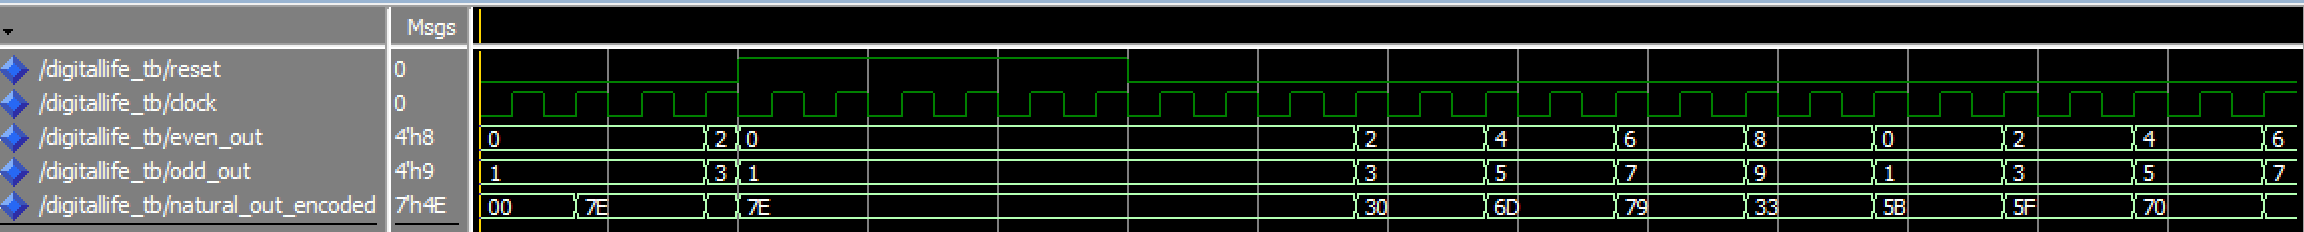
\includegraphics[width=\textwidth]{DL_Online_testbench.png}
    \caption{testbench对DigitalLife\_Online文件夹下的文件进行的仿真结果波形图 (放大后清晰可见)}
\end{figure}

\qquad 在上图中,可以看到随着clock信号每2次上升沿的出现(每2个时钟周期进行一次数列值的更新),
各个数列(奇数列、偶数列)都发生一次变化。在reset信号从0变为1时,
各信号回到了初始状态,reset信号从1变为0时,各信号继续随时钟变化而变化。其中最后一个信号为编码后的自然数数列,对应
没有译码的数码管使用,在本次仿真中其数值没有具体含义。\footnote{为什么图中第一次遇到2个上升沿时,波形没有变化?详见3.1中的说明。}


\subsection{JieLabs测试结果}
\qquad 见录屏文件JieLabsTest.mp4。在视频中展示了十六进制自然数数列、偶数列和奇数列。可看到大约每秒各数列都会发生变化。按下reset后可以看到各数列回到初始状态,不按reset时各信号随时钟变化而变化。


% \section{Experimental Data}

% \begin{tabular}{ll}
% Mass of empty crucible & \SI{7.28}{\gram}\\
% Mass of crucible and magnesium before heating & \SI{8.59}{\gram}\\
% Mass of crucible and magnesium oxide after heating & \SI{9.46}{\gram}\\
% Balance used & \#4\\
% Magnesium from sample bottle & \#1
% \end{tabular}

%----------------------------------------------------------------------------------------
%	SECTION 3
%----------------------------------------------------------------------------------------
\section{思考与总结}
\subsection{遇到的问题与解决方法}

\qquad 在我第一次仿真时,我遇到了奇怪的问题,即我在代码中设置为在clock信号上升沿时,更新数列和输出的值,但是得到的波形图却是在每次clk信号下降沿时
发生变化,这令我十分不解。在参考了StackOverflow的解答并且与吕志远助教交流后,我学习到一个process中signal赋值的过程,只会在process结束时一起执行,被赋予的
值是所有signal在process进行前的值,
即所有信号在本轮process中,值仍为上一轮的值。

\qquad 因此,在刚才发现的下降沿信号发生变化的问题中,出现上升沿时,该程序会进行数列临时变量的更新和输出信号的更新,但在上升沿结束时
输出信号仍然保持为上一轮的结果。在下降沿时,不会有数列临时变量的更新,有输出信号的更新,这时输出信号更新为了上升沿本意要更新的数值,
因此出现了在下降沿时信号变化而上升沿中信号不便的问题。出现该问题的代码和波形图如下,注意第27行的代码和上面的注释。

\begin{lstlisting}[language={vhdl}]
entity DigitalLife is
port (
    reset:in std_logic := '0';  
    clock:in std_logic := '0';  
    natural_out_hex: 
        out std_logic_vector(3 downto 0) := "0000"
);
end entity DigitalLife;
architecture bhv of DigitalLife is
    signal natural_seq_hex :
        std_logic_vector(3 downto 0) := "0000";
begin
    process (clock, reset) begin
        if (reset = '1') then
            natural_seq_hex <= "0000";
            natural_out_hex <= "0000";
        elsif (rising_edge(clock)) then
            if (natural_seq_hex = 15) then
                natural_seq_hex <= (others => '0'); 
            else
                natural_seq_hex <= natural_seq_hex +1;
            end if;
        end if;
    -- When falling edge, this also be activated and
    -- the value of the last rising edge
    -- is updated at falling edge.
    natural_out_hex <= natural_seq_hex;
    end process;
end architecture bhv;

\end{lstlisting}

\begin{figure}[h]
    \centering
    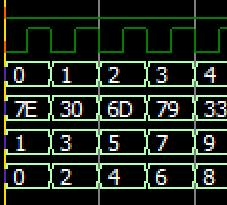
\includegraphics[]{fallingEdgeUpdate.jpg}
    \caption{下降沿时数据变化而上升沿时数据不变}
\end{figure}
\qquad 这个问题我通过将对输出信号的赋值加到了对于上升沿的判断分支中解决了,这样做不会在下降沿时触发赋值,只会在下一次上升沿时
对输出变量为上一次上升沿时的值。不过这样做也有一定的小问题,即在第一次遇到上升沿时,输出信号并不会变化,只会在第二次上升沿及其之后
发生规律的变化。这也解释了2.1.1和2.1.2中脚注提出的两个小疑问。

\subsection{一些感想与建议}
\qquad 非常感谢老师和助教在本次实验中给予我的帮助,无论是在群聊的答疑还是助教细心地与我私聊解决问题,都让我感受到了老师和助教的用心!

\qquad 不过在VHDL入门、testbench入门时,我感觉还是遇到了很大的困难。可能一方面我在面对生疏知识时接受没有那么迅速,另一方面可能也是
关于VHDL的网络资源不是特别丰富。有可能的话,建议老师和助教为新入门的同学准备更多的参考资料或者学习路线,以帮助同学们更好地掌握这门课的知识,享受数字逻辑实验的乐趣。



\section{参考资料}
1. RISING EDGE AND FALLING EDGE PROBLEM \\\url{https://stackoverflow.com/questions/50461404}


2. MODELSIM SIMULATION \\\url{https://blog.csdn.net/u013273161/article/details/82454134}


3. TESTBENCH TUTORIAL \\\url{https://vhdlguide.readthedocs.io/en/latest/vhdl/testbench.html#}


4. TESTBENCH CREATION \\\url{https://www.doulos.com/knowhow/perl/testbench_creation/}


5. HOW SIGNAL ASSIGNMENT WORK IN PROCESS \\\url{https://stackoverflow.com/questions/5060635/how-does-signal-assignment-work-in-a-process}


6. EXAMPLE PROGRAMS FOR VHDL \\ \url{https://www.cnblogs.com/uestcman/p/10202150.html}

% \section{Sample Calculation}

% \begin{tabular}{ll}
% Mass of magnesium metal & = \SI{8.59}{\gram} - \SI{7.28}{\gram}\\
% & = \SI{1.31}{\gram}\\
% Mass of magnesium oxide & = \SI{9.46}{\gram} - \SI{7.28}{\gram}\\
% & = \SI{2.18}{\gram}\\
% Mass of oxygen & = \SI{2.18}{\gram} - \SI{1.31}{\gram}\\
% & = \SI{0.87}{\gram}
% \end{tabular}

% Because of this reaction, the required ratio is the atomic weight of magnesium: \SI{16.00}{\gram} of oxygen as experimental mass of Mg: experimental mass of oxygen or $\frac{x}{1.31}=\frac{16}{0.87}$ from which, $M_{\ce{Mg}} = 16.00 \times \frac{1.31}{0.87} = 24.1 = \SI{24}{\gram\per\mole}$ (to two significant figures).

% %----------------------------------------------------------------------------------------
% %	SECTION 4
% %----------------------------------------------------------------------------------------

% \section{Results and Conclusions}

% The atomic weight of magnesium is concluded to be \SI{24}{\gram\per\mol}, as determined by the stoichiometry of its chemical combination with oxygen. This result is in agreement with the accepted value.

% \begin{figure}[h]
% \begin{center}
% 
\includegraphics[width=0.65\textwidth]{placeholder} % Include the image placeholder.png
% \caption{Figure caption.}
% \end{center}
% \end{figure}

% %----------------------------------------------------------------------------------------
% %	SECTION 5
% %----------------------------------------------------------------------------------------

% \section{Discussion of Experimental Uncertainty}

% The accepted value (periodic table) is \SI{24.3}{\gram\per\mole} \cite{Smith:2012qr}. The percentage discrepancy between the accepted value and the result obtained here is 1.3\%. Because only a single measurement was made, it is not possible to calculate an estimated standard deviation.

% The most obvious source of experimental uncertainty is the limited precision of the balance. Other potential sources of experimental uncertainty are: the reaction might not be complete; if not enough time was allowed for total oxidation, less than complete oxidation of the magnesium might have, in part, reacted with nitrogen in the air (incorrect reaction); the magnesium oxide might have absorbed water from the air, and thus weigh ``too much." Because the result obtained is close to the accepted value it is possible that some of these experimental uncertainties have fortuitously cancelled one another.

% %----------------------------------------------------------------------------------------
% %	SECTION 6
% %----------------------------------------------------------------------------------------

% \section{Answers to Definitions}

% \begin{enumerate}
% \begin{item}
% The \emph{atomic weight of an element} is the relative weight of one of its atoms compared to C-12 with a weight of 12.0000000$\ldots$, hydrogen with a weight of 1.008, to oxygen with a weight of 16.00. Atomic weight is also the average weight of all the atoms of that element as they occur in nature.
% \end{item}
% \begin{item}
% The \emph{units of atomic weight} are two-fold, with an identical numerical value. They are g/mole of atoms (or just g/mol) or amu/atom.
% \end{item}
% \begin{item}
% \emph{Percentage discrepancy} between an accepted (literature) value and an experimental value is
% \begin{equation*}
% \frac{\mathrm{experimental\;result} - \mathrm{accepted\;result}}{\mathrm{accepted\;result}}
% \end{equation*}
% \end{item}
% \end{enumerate}

%----------------------------------------------------------------------------------------
%	BIBLIOGRAPHY
%----------------------------------------------------------------------------------------

\bibliographystyle{apalike}

\bibliography{sample}

%----------------------------------------------------------------------------------------


\end{document}